\documentclass[a4paper, 11pt]{beamer}

\usepackage{polski}
\usepackage[utf8]{inputenc}

\mode<presentation> {
	\usetheme{Frankfurt}
	\setbeamercovered{transparent}
	\usecolortheme{default}
}

\title{Ekonometria Dynamiczna}
\subtitle{Szeregi czasowe: podstawowe definicje i miary}
\author{mgr Paweł Jamer\thanks{pawel.jamer@gmail.com}}

\begin{document}

	\begin{frame}
		\titlepage
	\end{frame}
	
	\section{Definicje}

	\begin{frame}{Proces Stochastyczny}
		\textbf{Niech:}
		\begin{itemize}
			\item $\left(\Omega, \mathcal{F}, \boldsymbol{P}\right)$ --- przestrzeń probabilistyczna;
			\item $\mathbb{T}$ --- zbiór indeksów (zwykle czas).
			\begin{itemize}
				\item $\mathbb{T} \subseteq \mathbb{Z}$ --- czas dyskretny.
				\item $\mathbb{T} \subseteq \mathbb{R}$ --- czas ciągły.
			\end{itemize}
		\end{itemize}
		
		\begin{block}{\textbf{Proces stochastyczny}}
			Procesem stochastycznym nazwiemy taką funkcję \[
				\left(t,\omega\right) \mapsto X_t\left(\omega\right), t \in \mathbb{T}, \omega \in \Omega,
			\]
			że dla każdego ustalonego $t\in\mathbb{T}:$ $X_t\left(\omega\right)$ jest zmienną losową.
		\end{block}
	\end{frame}
	
	\begin{frame}{Proces Stochastyczny}
		\begin{block}{\textbf{Proces stochastyczny}}
			Procesem stochastycznym nazwiemy taką funkcję \[
				\left(t,\omega\right) \mapsto X_t\left(\omega\right), t \in \mathbb{T}, \omega \in \Omega,
			\]
			że dla każdego ustalonego $t\in\mathbb{T}:$ $X_t\left(\omega\right)$ jest zmienną losową.
		\end{block}
		
		\begin{alert}{\textbf{Uwaga.}}
			Wyżej zdefiniowany proces stochastyczny oznaczać będziemy zazwyczaj pisząc $X_t$ albo $\left\{X_t\right\}$ lub używając zapisu
			akcentującego zakres indeksów postaci $\left\{X_t\right\}_{t\in\mathbb{T}}$ albo $\left\{X_t\right\}_{t=1}^{\infty}.$
		\end{alert}
		
		\textbf{Oznaczenia:}
		\begin{itemize}
			\item $\mathcal{S}=\left\{X_t\left(\omega\right): t\in\mathbb{T}, \omega\in\Omega\right\}$ --- przestrzeń stanów.
			\item $s\in\mathcal{S}$ --- stan procesu.
			\item $t \mapsto X_t\left(\omega\right)$ --- trajektoria (realizacja) procesu.
		\end{itemize}
	\end{frame}
	
	\begin{frame}{Szereg Czasowy}
		\begin{block}{\textbf{Szereg czasowy}}
			Szeregiem czasowym nazywamy proces stochastyczny $X_t,$ którego zbiór indeksów $\mathbb{T}$ reprezentuje czas.
		\end{block}
		
		\begin{alert}{\textbf{Uwaga.}}
			Wiele źródeł definiuje szereg czasowy jako \textit{realizację} procesu stochastycznego, którego zbiór indeksów $\mathbb{T}$ reprezentuje czas.
		\end{alert}
		
		\begin{alert}{\textbf{Uwaga.}}
			Będziemy rozpatrywać przede wszystkim przypadek $\mathbb{T} = \mathbb{Z}_+,$ zakładając niejawnie taktowanie tym samym odcinkiem czasowym.
			W praktyce zdarzają się odstępstwa od tego założenia (np. notowania giełdowe).
		\end{alert}
		
	\end{frame}
	
	\begin{frame}{Przykład (biały szum)}
		Szereg czasowy $\epsilon_t$ niezależnych zmiennych losowych o tym samym rozkładzie taki, że \begin{eqnarray*}
			\mathbb{E}\left(\epsilon_t\right) & = & 0,\\
			\mbox{Var}\left(\epsilon_t\right) & = & \sigma^2
		\end{eqnarray*} nazywać będziemy \textbf{białym szumem} i oznaczać $\mbox{WN}\left(0, \sigma^2\right)$.
		
		\begin{center}
			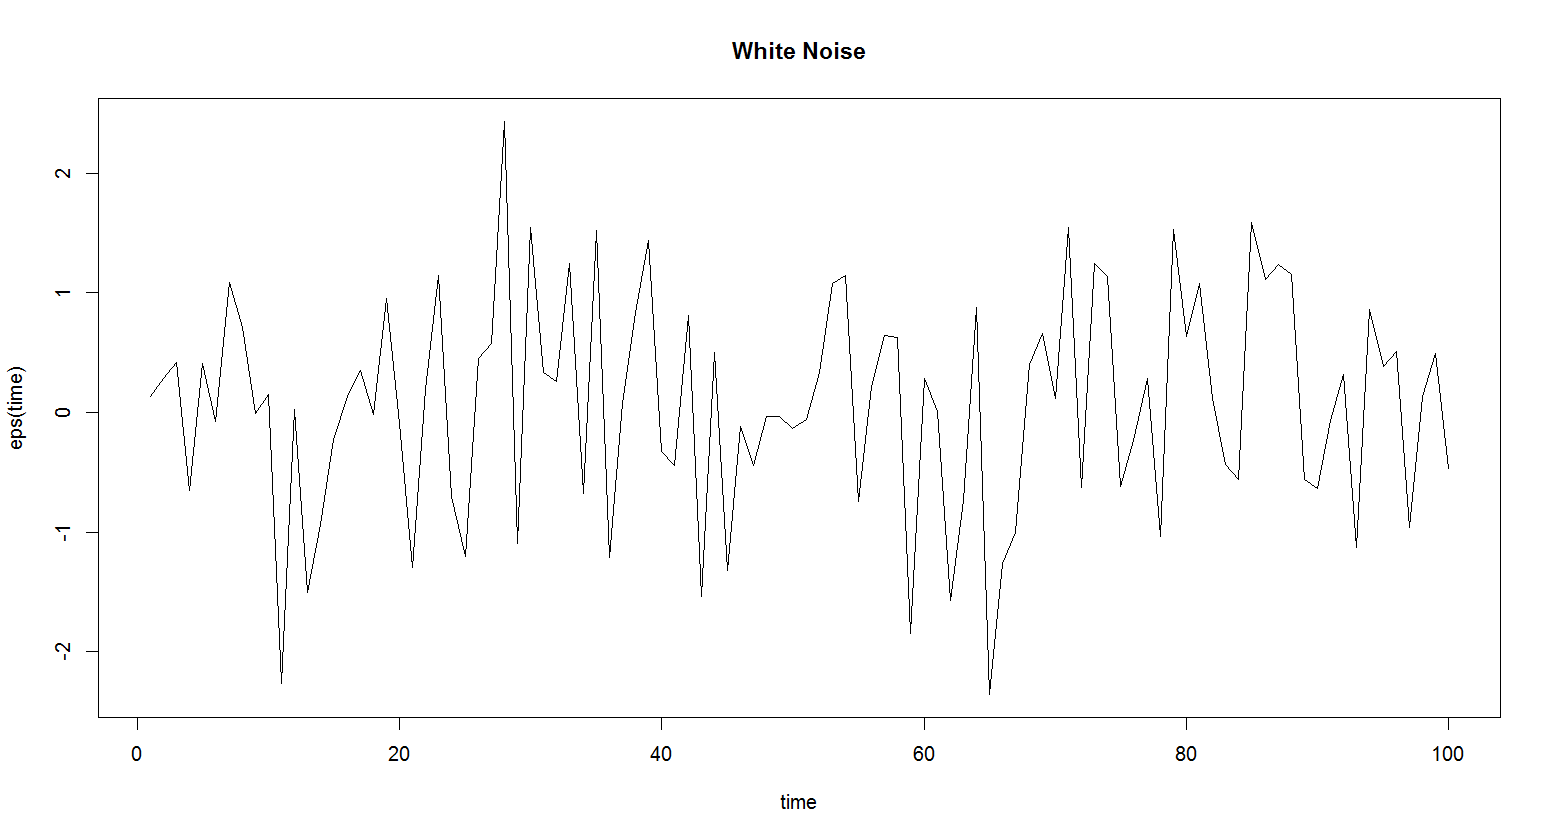
\includegraphics[scale=0.25]{./gfx/white_noise}
		\end{center}
	\end{frame}

	\begin{frame}{Przykład (model autoregresyjny)}
		Szereg czasowy \[
			X_t = \rho X_{t-1} + \epsilon_t,
		\] gdzie $\epsilon_t \sim \mbox{WN}\left(0, \sigma^2\right),$ nazwiemy szeregiem \textbf{autoregresyjnym rzędu 1} i oznaczymy $\mbox{AR}\left(1\right).$
		
		\begin{center}
			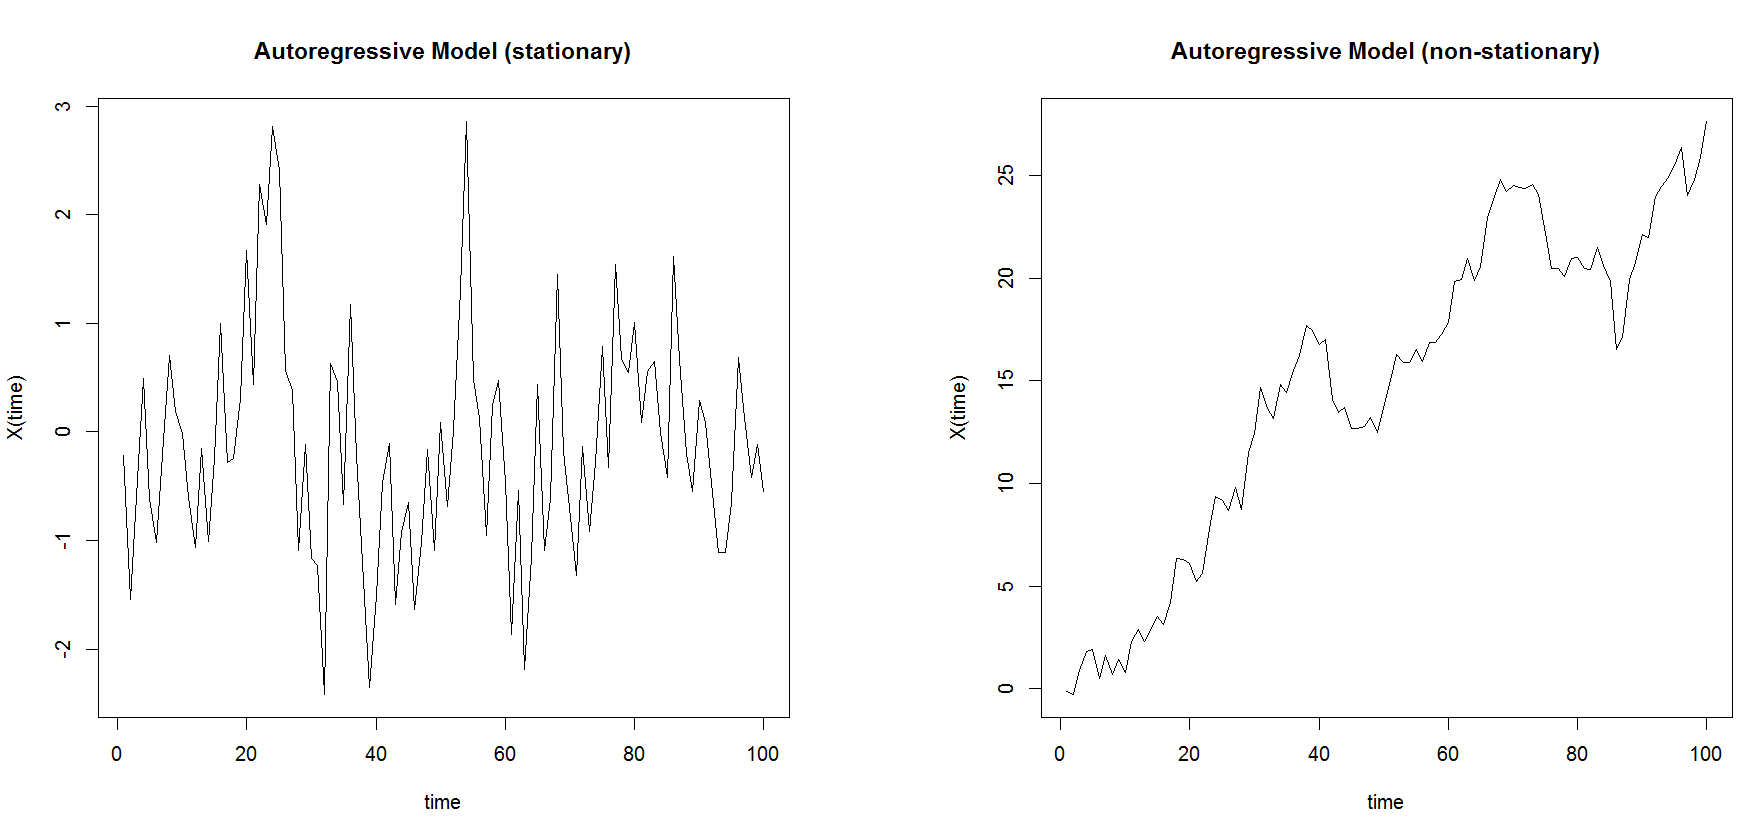
\includegraphics[scale=0.25]{./gfx/ar_1}
		\end{center}
	\end{frame}

	\section{Podstawowe miary}

	\begin{frame}{Wartość oczekiwana}
		\begin{block}{\textbf{Wartość oczekiwana}}
			Wartością oczekiwaną procesu stochastycznego $X_t$ nazywamy funkcję \[
				t \mapsto \mathbb{E}\left(X_t\right)
			\]
			o ile dla każdego $t\in\mathbb{T}:$ $\mathbb{E}\left|X_t\right| < \infty.$
		\end{block}
		
		\textbf{Niech:} $c$ - stała, $X,Y$ - zmienne losowe.
		
		\textbf{Właściwości:}
		\begin{itemize}
			\item $\mathbb{E}\left(c\right) = c,$
			\item $\mathbb{E}\left(cX\right) = c\mathbb{E}\left(X\right),$
			\item $\mathbb{E}\left(X+Y\right) = \mathbb{E}\left(X\right) + \mathbb{E}\left(Y\right),$
			\item $X,Y$ - niezależne $\Rightarrow$ $\mathbb{E}\left(XY\right) = \mathbb{E}\left(X\right) \mathbb{E}\left(Y\right).$
		\end{itemize}
	\end{frame}
	
	\begin{frame}{Wariancja}
		\begin{block}{\textbf{Wariancja}}
			Wariancją procesu stochastycznego $X_t$ nazywamy funkcję \[
				t \mapsto \mbox{Var}\left(X_t\right)
					= \mathbb{E}\left(X_t - \mathbb{E}\left(X_t\right)\right)^2
			\]
			o ile dla każdego $t\in\mathbb{T}:$ $\mathbb{E}\left(X_t^2\right) < \infty.$
		\end{block}
		
		\textbf{Niech:} $c$ - stała, $X,Y$ - zmienne losowe.
		
		\textbf{Właściwości:}
		\begin{itemize}
			\item $\mbox{Var}\left(c\right) = 0,$
			\item $\mbox{Var}\left(cX\right) = c^2 \mbox{Var}\left(X\right),$
			\item $\mbox{Var}\left(X + c\right) = \mbox{Var}\left(X\right),$
			\item $\mbox{Var}\left(X \pm Y\right) = \mbox{Var}\left(X\right) + \mbox{Var}\left(Y\right) \pm 2 \mbox{Cov}\left(X,Y\right),$
			\item $X,Y$ - niezależne $\Rightarrow$ $\mbox{Var}\left(X \pm Y\right) = \mbox{Var}\left(X\right) + \mbox{Var}\left(Y\right).$
		\end{itemize}
	\end{frame}
	
	\begin{frame}{Kowariancja}
		\begin{block}{\textbf{Kowariancja}}
			Kowariancją procesów stochastycznych $X_t$ i $Y_t$ nazwiemy funkcję \[
				\left(s,t\right) \mapsto \mbox{Cov}\left(X_s, Y_t\right)
					= \mathbb{E}\left(X_s - \mathbb{E}\left(X_s\right)\right)\left(Y_t - \mathbb{E}\left(Y_t\right)\right)
			\]
			o ile dla każdego $t\in\mathbb{T}:$ $\mathbb{E}\left(X_t^2\right) < \infty$ oraz $\mathbb{E}\left(Y_t^2\right) < \infty.$
		\end{block}
		
		\begin{alert}{\textbf{Uwaga.}}
			Kowariancja wyraża siłę zależności liniowej występującej pomiędzy dwiema zmiennymi losowymi.
			\begin{itemize}
				\item $X, Y$ - liniowo niezależne $\Leftrightarrow$ $\mbox{Cov}\left(X, Y\right) = 0,$
				\item $X, Y$ - niezależne $\Rightarrow$ $\mbox{Cov}\left(X, Y\right) = 0,$
				\item $X, Y$ - niezależne $\not\Leftarrow$ $\mbox{Cov}\left(X, Y\right) = 0.$
			\end{itemize}
		\end{alert}
		
		\begin{alert}{\textbf{Uwaga.}}
			Kowariancję procesu stochastycznego $X_t$ z samym sobą nazywamy \textbf{autokowariancją} i
			oznaczymy symbolem $\gamma_X\left(s,t\right).$
		\end{alert}
	\end{frame}
	
	\begin{frame}{Korelacja}
		\begin{block}{\textbf{Korelacja}}
			Korelacją procesów stochastycznych $X_t$ i $Y_t$ nazwiemy funkcję \[
				\left(s,t\right) \mapsto \mbox{Corr}\left(X_s, Y_t\right)
					= \frac{\mbox{Cov}\left(X_s, Y_t\right)}{\sqrt{\mbox{Var}\left(X_s\right)}\sqrt{\mbox{Var}\left(Y_t\right)}}
			\]
			o ile dla każdego $t\in\mathbb{T}:$ $\mathbb{E}\left(X_t^2\right) < \infty$ oraz $\mathbb{E}\left(Y_t^2\right) < \infty.$
		\end{block}
		
		\begin{alert}{\textbf{Uwaga.}}
			Korelacja jest unormowaną miarą zależności liniowej łączącej dwie zmienne losowe.
			\begin{itemize}
				\item $\mbox{Corr}\left(X, Y\right) = 1$ $\Rightarrow$ pełna dodatnia zależność liniowa,
				\item $\mbox{Corr}\left(X, Y\right) = 0$ $\Rightarrow$ brak zależności liniowej,
				\item $\mbox{Corr}\left(X, Y\right) = -1$ $\Rightarrow$ pełna ujemna zależność liniowa.
			\end{itemize}
		\end{alert}
		
		\begin{alert}{\textbf{Uwaga.}}
			Korelację procesu stochastycznego $X_t$ z samym sobą nazywamy \textbf{autokorelacją} i oznaczymy symbolem $\rho_X\left(s,t\right).$
		\end{alert}
	\end{frame}

	\section*{}

	\begin{frame}
		\center
		\Huge \bfseries
		Pytania?
	\end{frame}

	\begin{frame}
		\center
		\Huge \bfseries
		Dziękuję za uwagę!
	\end{frame}

\end{document}